\section{Conexões entre neurônios}
\subsection{Sinapses}
\begin{frame}{Sinapses}
	\begin{columns}[t]
		\column{5cm}
			\begin{figure}[tb]
				\centering
				\caption{Esquema simplificado de uma sinapse química}
				\label{fig:sinapses}
				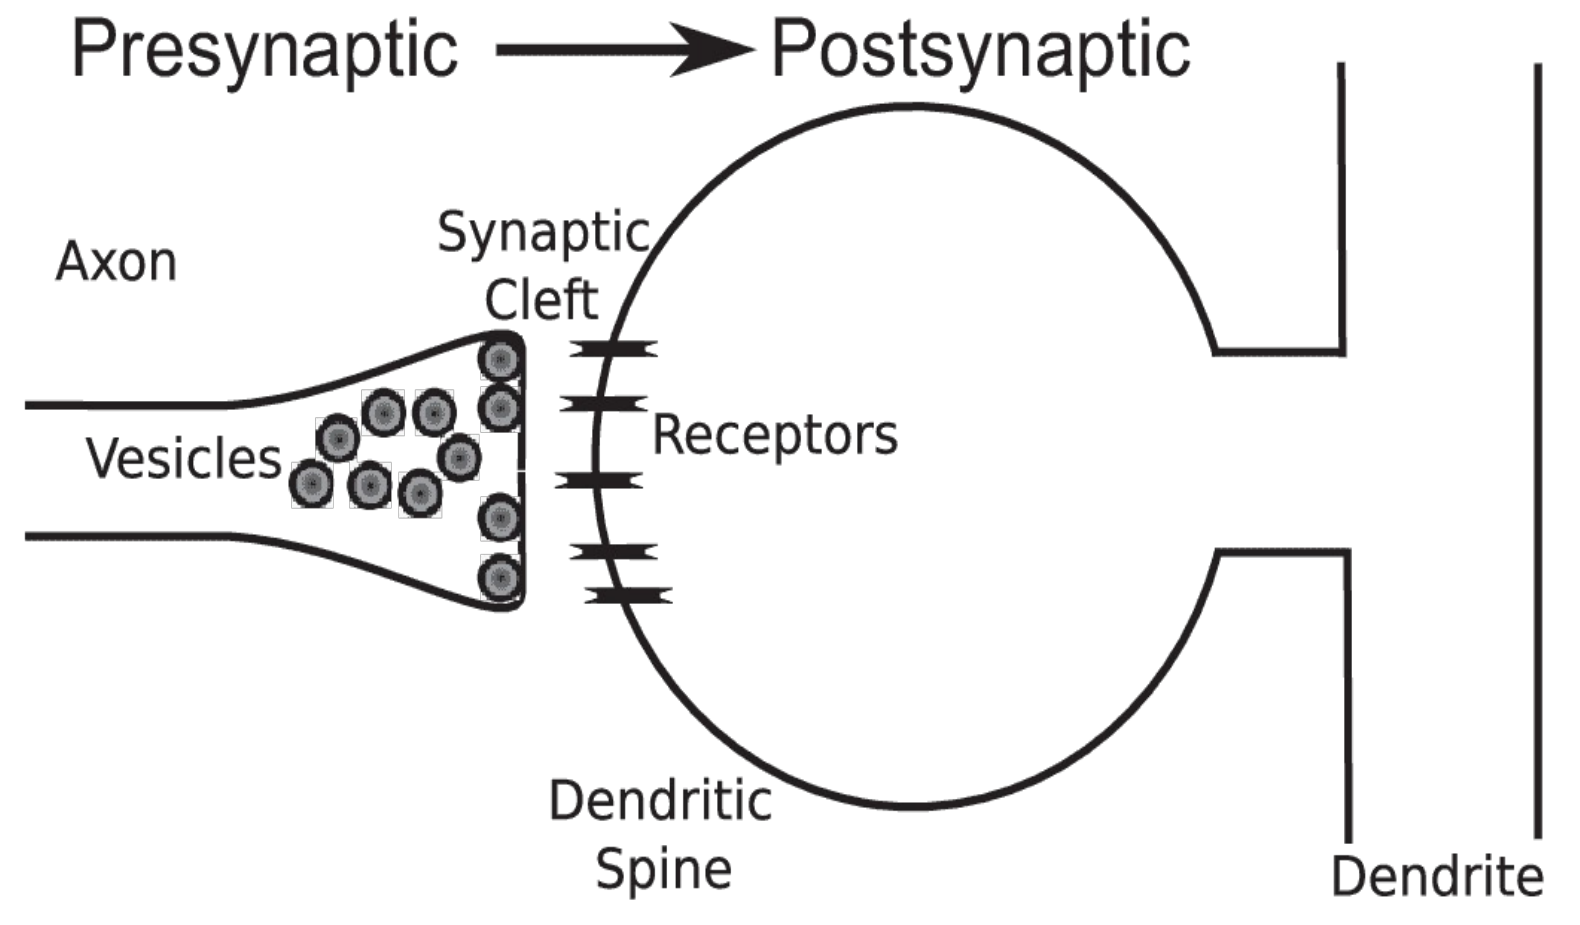
\includegraphics[width=0.9\linewidth]{figs/sinapses}\\
%				\fonte{\cite{miller_introductory_2018}}
				%TODO: trocar figura
			\end{figure}
		\column{5cm}
			\begin{itemize}
				\item Conexão entre dois neurônios;
				\item elétricas: se dão a partir de uma junção entre duas células;
				\item químicas: conectadas por um espaço entre as células por meio de neurotransmissores.
				\item excitatórias: despolarizam a membrana; inibitórias: hiperpolarizam
				\note{glutamato: excita a célula}
				\note{gaba: normalmente inibe}
			\end{itemize}
	\end{columns}
\end{frame}

\begin{frame}{Sinapses}
	\begin{columns}[t]
		\column{5cm}
			\begin{figure}[tb]
				\centering
				\caption{Condutância sináptica em resposta aos potenciais de ação da célula pré-sináptica}
				\label{fig:respostasinaptica}
				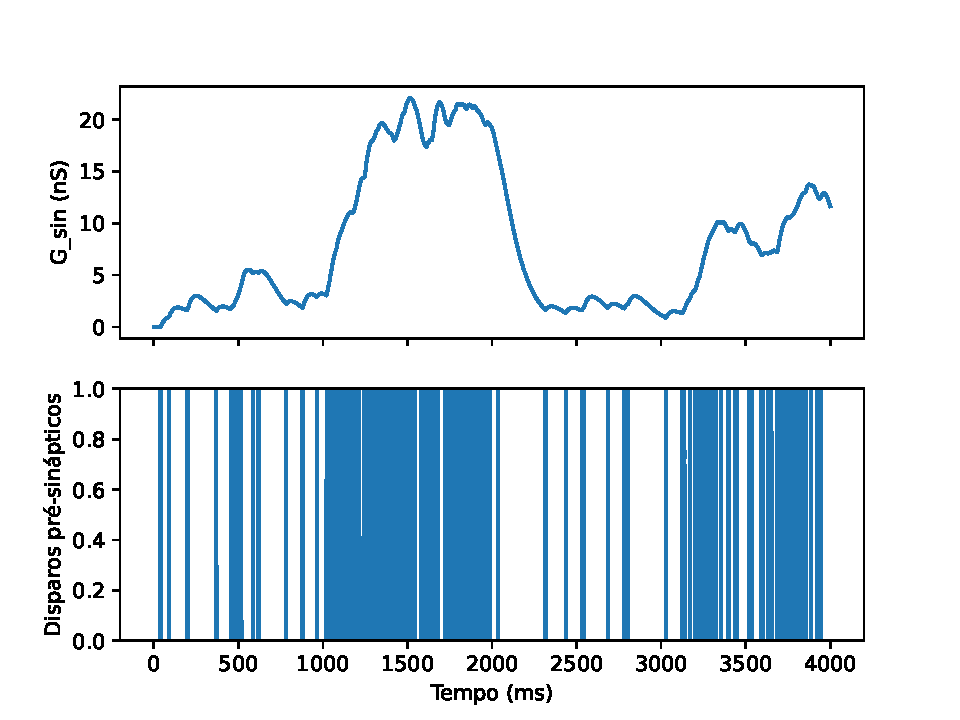
\includegraphics[width=0.9\linewidth]{figs/resposta_sinaptica}
%				\fonte{O autor (\the\year)}
				%TODO: regerar
			\end{figure}
		\column{5cm}
			\[
				\frac{dG_{sin}(t)}{dt}=\frac{-G_{sin}(t)}{\tau_{sin}}
			\]\[
				G_{sin}(t)\mapsto G_{sin}(t)+\Delta G
			\]
			\begin{itemize}
				\item $G_{sin}(t)$: condutância sináptica
				\item $\tau_{sin}$: constante de tempo
				\item $\Delta G$: incremento de condutância
			\end{itemize}
	\end{columns}
\end{frame}

\begin{frame}{Sinapses dinâmicas}
	\begin{columns}[t]
		\column{5cm}
			\begin{figure}[tb]
				\centering
				\caption{Depressão e facilitação sináptica}
				\label{fig:plasticidadecurtaduracao}
				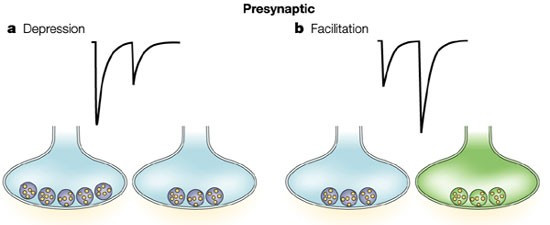
\includegraphics[width=0.9\linewidth]{figs/plasticidade_curta_duracao}
%				\fonte{Adaptado de \cite{blitz_short-term_2004}}
				%TODO: trocar figura
			\end{figure}
		\column{5cm}
		\begin{itemize}
			\item Depressão de curta duração: redução temporária na força sináptica;
			\item Facilitação de curta duração: incremento temporário na força sináptica
		\end{itemize}
	\end{columns}
	\[
		\begin{aligned}
			\frac{dD}{dt}&=\frac{1-D}{\tau_D} &\qquad &D\mapsto D-p_0FD\\
			\frac{dF}{dt}&=\frac{1-F}{\tau_F} &\qquad &F\mapsto F+f_{fat}(F_{max}-F)
		\end{aligned}
		\qquad\qquad \Delta G=G_{max}p_0FD
	\]
\end{frame}

\subsection{Multi-estabilidade}

\subsection{Modelos de taxa de disparo}

\subsection{Aprendizado e plasticidade de longa duração}
